\documentclass[tikz,border=3mm]{standalone}
\usepackage{booktabs}

\begin{document}

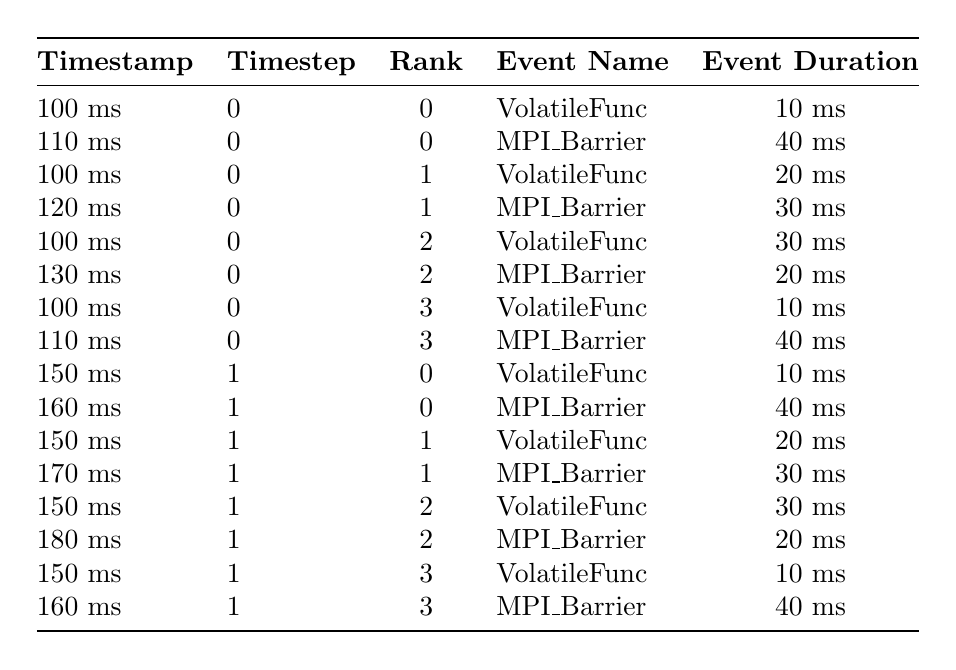
\begin{tikzpicture}
\node[anchor=north west] at (0,0) {
\begin{tabular}{@{}llclc@{}}
\toprule
\textbf{Timestamp} & \textbf{Timestep} & \textbf{Rank} & \textbf{Event Name} & \textbf{Event Duration} \\ 
\midrule
100 ms & 0 & 0 & VolatileFunc & 10 ms \\
110 ms & 0 & 0 & MPI\_Barrier & 40 ms \\
100 ms & 0 & 1 & VolatileFunc & 20 ms \\
120 ms & 0 & 1 & MPI\_Barrier & 30 ms \\
100 ms & 0 & 2 & VolatileFunc & 30 ms \\
130 ms & 0 & 2 & MPI\_Barrier & 20 ms \\
100 ms & 0 & 3 & VolatileFunc & 10 ms \\
110 ms & 0 & 3 & MPI\_Barrier & 40 ms \\
150 ms & 1 & 0 & VolatileFunc & 10 ms \\
160 ms & 1 & 0 & MPI\_Barrier & 40 ms \\
150 ms & 1 & 1 & VolatileFunc & 20 ms \\
170 ms & 1 & 1 & MPI\_Barrier & 30 ms \\
150 ms & 1 & 2 & VolatileFunc & 30 ms \\
180 ms & 1 & 2 & MPI\_Barrier & 20 ms \\
150 ms & 1 & 3 & VolatileFunc & 10 ms \\
160 ms & 1 & 3 & MPI\_Barrier & 40 ms \\
\bottomrule
\end{tabular}
};
\end{tikzpicture}

\end{document}